%====================================================================================================
% Controle PID
%====================================================================================================
% Plano de Trabalho
%----------------------------------------------------------------------------------------------------
% Autor			: Kelvim Rodrigues de Oliveira	
% Orientador		: Gedson Faria
% Instituição 		: UFMS - Universidade Federal do Mato Grosso do Sul
% Unidade		: CPCX - Campus de Coxim
%----------------------------------------------------------------------------------------------------
% Arquivo		: plano_trab_kelvim.tex
% Data de criação	: 13 de Maio de 2017
%====================================================================================================

\documentclass[a4paper,12pt,portuguese]{ufms-cpcx}


\usepackage{float}
\usepackage{xcolor}
\usepackage{listings}
\usepackage[utf8]{inputenc}
\usepackage[top=30mm,bottom=25mm,left=25mm,right=20mm]{geometry}
\usepackage{pdfpages}
\usepackage [onehalfspacing]{setspace} 
\usepackage{indentfirst}
%\usepackage{caption}
\usepackage[font=small]{caption}
\usepackage{subcaption}
\usepackage{multicol}
\usepackage{booktabs}	% http://ctan.org/pkg/booktabs
\usepackage{array}	% http://ctan.org/pkg/array

\newcolumntype{M}{>{\centering\arraybackslash}m{\dimexpr.25\linewidth-2\tabcolsep}}

\lstset{
	language=C++,
	basicstyle=\ttfamily\small, 
	keywordstyle=\color{blue}, 
	stringstyle=\color{verde}, 
	commentstyle=\color{red}, 
	extendedchars=true, 
	showspaces=false, 
	showstringspaces=false, 
	numbers=left,
	numberstyle=\tiny,
	breaklines=true, 
	backgroundcolor=\color{green!10},
	breakautoindent=true, 
	captionpos=b,
	xleftmargin=0pt,
}

\begin{document}
\definecolor{verde}{rgb}{0,0.5,0}
\thispagestyle{empty}



\titulo{ Plano de Trabalho\vskip 1.5cm 
	Controle de velocidade utilizando P.I.D. }\vskip 0.5cm
\autor{Kelvim Rodrigues de Oliveira}

\orientacao{Prof. Doc. Gedson Faria}
%\docarea{Bacharelado em Sistemas de Informação}
\textofree{\large Bacharelado em Sistemas de Informação}

\vfill \centerline{
\includegraphics[scale=0.15]{figuras/ufms-logo.jpg}}

\vskip 0.5cm
\begin{center}
	Universidade Federal de Mato Grosso do Sul\\ 
	Campus de Coxim\\ \vskip 1.0cm
	13 de Maio de 2017
\end{center}

\chapter*{}

\begin{center}
	
	\begin{minipage}[t]{10cm}
		\begin{center}
			\vspace{-2cm}
			{{\Large Controle de velocidade utilizando P.I.D.}}  
		\end{center}
	\end{minipage}
	
\end{center}

\vskip 3.0cm \textofree{\large Plano de Trabalho}

\begin{flushright}
	\vspace{12cm}
	Coxim, 13 de Maio de 2017.
\end{flushright}

%\vspace{2cm}



%\tableofcontents

%\printglossaries

%\cleardoublepage
%\phantomsection
%\addcontentsline{toc}{chapter}{Lista de Tabelas}
%\listoftables



\chapter{Introdução}
Bla bla bla
 
 
 \section{Justificativa}  
 Bla bla bla


 \section{Objetivos}
 
 
 \section{Objetivo Geral}  
  
 O objetivo deste trabalho é estudar e implementar controle de velocidade entre os motores esquerdo e direito do robô jogador. 

\section{Objetivos Específicos}

\begin{itemize}
	%lista de itens	
	
	\item Criar uma interface simples e intuitiva para que qualquer pessoa sem alto nível de conhecimento no pacote \textit{Vaucanson-G} possa utilizá-lo.
	
	\item Desenvolver o sistema de transição livre.
	
	\item Desenvolver o sistema de transição dupla.
	
	
\end{itemize}

\section {Organização da Monografia}

\chapter{Revisão da Literatura}

\chapter{Futebol de robôs}
Este capitulo destina-se alguns conceitos, informações e história do futebol de robôs, suas principais modalidades, dinâmica de jogo e movimentos.

\section{Uma breve história sobre futebol de robôs}
Com duas organizações de referencia mundial para o estudo e organização quanto ao futebol de robôs, são elas a FIRA, sigla em inglês para Federation of International Robot-soccer Association e a RoboCup associaçães que tem como objetivo promover pesquisas nas áreas de robótica e inteligência artificial, colaborando na divulgação científica através atividades afim de estimular o interesse dos participantes a resolver problemas. 

A FIRA, a qual foi fundada no ano de 1995, pelo professor Kim Jong-Hwan, realizou seu primeiro campeonato mundial na Coréia, em 1997, dois anos após sua fundação, com o objetivo de levar aos leigos e as gerações jovens o espírito da ciência e tecnologia aplicada à robótica. Desde então a FIRA vem realizando diversos eventos em vários
países do mundo, incluindo nossa pátria, o que fez com que o futebol de robôs obtivesse reconheci-mento mundial. Então o Brasil, que teve a oportunidade de sediar a Copa do Mundo em agosto de 1999, realizada entre os dias 4 a 8, na cidade Campinas no estado de São Paulo.

A RoboCup Criada no Japão por meio da iniciativa de um grupo de pesquisadores que tinham como objetivo em comum, o jogo de futebol, afim de promover o crescimento da ciência e tecnologia. De forma independente, os professores Minoru Asada,da Universidade de Osaka, e a Professora Manuela Veloso junto a seu aluno Peter Stone da Universidade Carnegie Mellon, EUA, estavam também trabalhando em robôs jogadores de futebol.
O primeiro campeonato da Robocup junto a primeira conferência, foram realizados em 1997. Onde compareceram mais de 40 equipes e mais de 5.000 espectadores. Infelizmente no Brasil até o momento não foram realizados eventos da Robocup com âmbito mundial.

\section{Modalidade} %subtitulo
Assim como o futebol jogado por humanos, o futebol de robôs também tem suas regras de jogo bem definidas. A FIRA Cup é um evento organizado com competições várias categorias, destacam-se as categorias Micro-Robot Soccer Tournament (MiroSot) e a Humanoid Robot Soccer Tournament (HuroSot), ambas são disputadas sob o olhar de um árbitro humano, já a categoria Simulated Robot Soccer Tournament (SimuroSot), que como o próprio nome sugere, trata-se de uma modalidade de simulação, quando não se tem a disposição de os recursos de hardware referentes aos robôs.

Este trabalho tem como foco o estudo das velocidades dos motores da categoria MiroSot. O acrônimo MiroSot, vem da denominação Micro Robot Soccer Tournament, cuja categoria é voltada para partidas com pequenos robôs que se movimentam através de dois motor, um motor para cada roda, realizando movimentos rápidos, enviados a partir de um computador disposto com uma inteligencia artificial com suas estratégias. Sendo este o ambiente principal do trabalho.
A partida deve ser jogada por duas equipes, com três robôs cada, um robô pode atuar como goleiro de acordo com as estratégias, já fora de campo o time contem três membros humanos, o "gerente", o "técnico" e um "instrutor" os quais só tem acesso ao palco. Cada equipe possui seu computador o qual é principalmente dedicado ao processamento de visão, identificação e de localização.  
O tamanho dos robôs desta categoria é limitado a 7,5 cm x 7,5 cm x 7,5 cm, altura da antena não deve ser considerada na medição do tamanho de um robô, é utilizado uma bola de golfe de cor laranja afim de facilitar o processo de visão computacional.
Esta categoria conta com duas ligas, a "Large league" (Liga grande) considerado grande pois o seu campo possui as dimensões de 400cm x 280cm e a "Middle league" (Liga média) que tem seu campo menor com as dimensões de 220cm x 180cm.

======== INSERIR IMAGEM DAS DIMENSÕES DO CAMPO =========


\chapter{Controlador PID}
== https://www.citisystems.com.br/controle-pid/ ===
Neste capítulo, explanarei sobre o controle PID -que é abreviatura para Proporcional, Integral e Derivativo- e como utiliza-lo em aplicações de controle que requerem um controle de precisão. Começaremos pelo exemplo onde um carro tenta manter uma distancia X do carro da frente.

\section{P - Proporcional}
Ao tentar manter uma distancia X o carro de trás deve acelerar proporcionalmente quando o carro da frente acelerar e começar a distanciar, tentando alcançar o mesmo. No entanto, caso o carro de trás venha acelerar mais que o carro da frente a distancia será menor que a desejada, X, então a nova correção é frear para aumentar a distancia buscando a distancia desejada de X. Novamente caso a correção, que desta vez é a frenagem(desaceleração), for muito, a sua distancia se será superior a distancia desejada de X, então novamente terá de acelerar. Isso ocorrera indefinitivamente caso a aceleração não proporcional não esteja correta, ou seja, acelerando de mais e freando de menos e não atingindo o ponto alvo(set point). Então esta aceleração é chapada de ganho ou proporcional(P) em um controle PID.

\section{I - Integral}
A integral, neste exemplo dos carros, seria como recuperar a distancia X a cada instante, caso o veiculo da frente venha a acelerar, o veiculo de trás acelera gradualmente afim de atingir a distancia X com mais suavidade, este procedimento pode ser comparado a integral de um controle PID.

\section{D - Derivativo}
A derivada é utilizada para eliminar erros acumulados na integral, neste exemplo dos carros, seria quando o carro de trás percebe que a distancia desce ou decresce muito rapidamente em relação a desejada X, deixando as correções da integral ainda mais suaves, diminuindo a oscilação das correções em volta do Setpoint.

\chapter{Ambiente de desenvolvimento}
Este capítulo aborda as ferramentas utilizadas para o desenvolvimento da programação dos robôs jogadores. O sistema operacional escolhido foi o Ubuntu Gnome 17.04 64-bit, por ser uma distribuição linux o Ubuntu já possui os drivers USB para comunicação a placas de teste, a utilizada no projeto foi a placa Arduino Nano 328, com o driver USB, como o FTDI. Sera descrito também neste capítulo a instalação e configuração dos softwares: IDE Arduino, IDE Clion 2017.1 e PlatformIO.

\section{Arduino IDE}\label{arduinoide}
======== https://www.arduino.cc/en/main/software ===
O Arduino 1.8.3(IDE) é um software open-source para desenvolvimento de programas para Arduino. A utilização deste software torna fácil escrever códigos e subir(upload) para a placa. O Arduino IDE tem suporte para Windows, Mas OS e para Linux. Ambiente foi desenvolvido em Java baseado no Processing e outros softwares open-source, com a utilização da IDE qualquer placa Arduino pode ser utilizada com poucas configurações.

\subsection{Intalação}
Na pagina oficial de download https://www.arduino.cc/en/Main/Software foi realizado o download conforme o sistema operacional, neste caso, Linux x64, ao selecionar o download é possível fazer uma doação para os desenvolvedores da IDE, visto que é um projeto open-source e software livre, não tendo fins lucrativos, o mesmo depende dessa colaboração da comunidade para permanecer ativo e continuar expandido. Então realizado o download da versão atual, neste momento a versão 1.6.10 para linux.

\begin{figure}[H]	
	\centering
	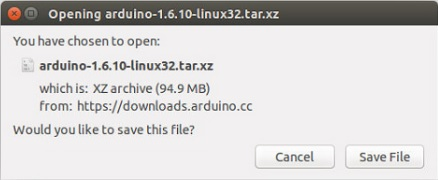
\includegraphics[width=0.5\textwidth]{dlArduino.jpg}
	\caption{Titulo.}
\end{figure}
Ao finalizar o download do arquivo compactado, sera necessário descompactar em um diretório desejado, este ainda não sera o diretório de instalação. 
\begin{figure}[H]	
	\centering
	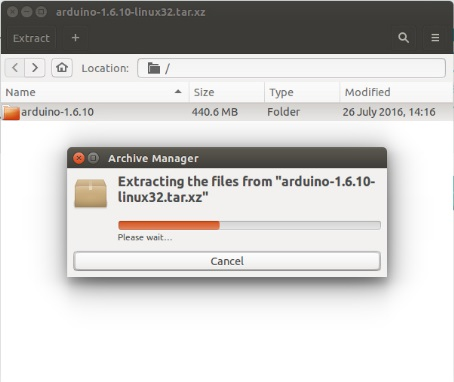
\includegraphics[width=0.5\textwidth]{unrarArduino.jpg}
	\caption{Titulo.}
\end{figure}
Abrindo o terminal navegue pelos diretórios utilizando o comando ‘CD’ até o diretório arduino-1.6.x o qual foi criado ao descompactar o arquivo. Execute então o arquivo ‘intall.sh’ utilizando o comando: 
\begin{lstlisting}
./install.sh
\end{lstlisting}
O processo de instalação é rápido, um novo ícone foi criado na área de trabalho.
\begin{figure}[H]	
	\centering
	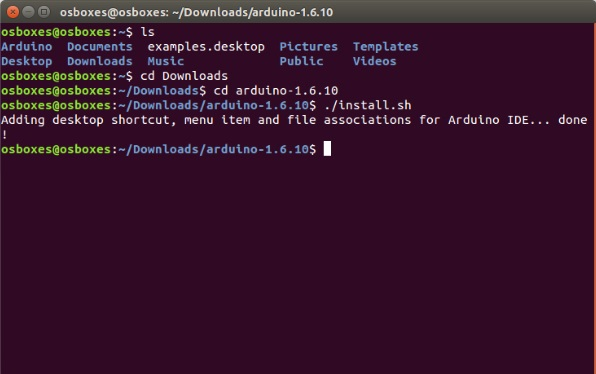
\includegraphics[width=0.5\textwidth]{installArduino.jpg}
	\caption{Titulo.}
\end{figure}

\section{Clion 2017.1}
====== https://www.jetbrains.com/clion/ =======
CLion é uma IDE multi-plataforma, criada pela empresa JetBrains para desenvolvimento de softwares nas linguagens C e C++, uma ferramenta poderosa. Suporte as linguagens nativas C e C++, incluindo C++11, C++14, libc++ e mais. A ferramenta desenvolvimento conta com ótimos recursos tais como: navegação, geração de código, gerenciamento de bibliotecas entre outros.
\subsection{Instalação}
Na página oficial de download do Clion ``https://www.jetbrains.com/clion/download/\#\=linux" foi realizado o download do arquivo ``CLion-*.tar.gz" da versão compatível com o sistema operacional. Descompacte o arquivo ``CLion-*.tar.gz", neste projeto foi descompactado no diretório /opt, sendo assim foi utilizado o seguinte comando para descompactar direto no diretório desejado.
\begin{lstlisting}
sudo tar xf CLion-*.tar.gz -C /opt/
\end{lstlisting}
Ao finalizar a descompactação, novamente navegue até o diretório /bin, diretório este que se encontra junto aos arquivos descompactados, utilizando o comando: 
\begin{lstlisting}
cd /opt/CLion-*/bin
\end{lstlisting}
Execute o arquivo clion.sh que se encontra dentro do subdiretório /bin, com o comando:
\begin{lstlisting}
./clion.sh
\end{lstlisting}

\section{PlatformIO}
Diferente microcontroladores normalmente exigem diferentes ferramentas de desenvolvimento, para o Arduino temos a Arduino IDE. Outros usuários preferem ferramentas com auxílios. Tais ambientes de desenvolvimentos como o Eclipse, o qual trás recursos que ajudam a gerenciar seus projetos, bibliotecas e funções de autocompletar. As vezes é um pouco difícil manter-se na linha com diferentes microcontroladores e ferramentas. Então o ecossistema (como é chamado pelos seus desenvolvedores) open-source do PlatformIO junta tudo em uma única ferramenta. Sendo uma ferramenta multiplataforma podendo ser instalada nos sistemas operacionais Linux, Windows e MAC, dá suporte ao compilação para mais de 200 placas de teste, com mais de 15 plataformas de desenvolvimento e 10 frameworks, cobrindo então as placas mais populares do mercado, fazendo o trabalho duro de organização de centenas de projeto e bibliotecas que podem ser incluídas no projeto.
\subsection{Instalação}
A instalação ou atualização no MAC e Linux é feita pelo terminal de um modo muito fácil, apenas utilizando o comando(sudo pode ser requerido): 
\begin{lstlisting}
python -c "$(curl -fsSL https://raw.githubusercontent.com/platformio/platformio/master/scripts/get-platformio.py)"
\end{lstlisting}

\section{Iniciando um novo projeto}
Para criar um novo projeto primeiramente devemos abrir a IDE Clion, deve-se criar um novo projeto na linguagem C++ clicando no File, New Poject então em Create. Ao finalizar a criação do novo projeto, abra as opções de configurações utilizando o atalho de teclado ``Ctrl + Alt + S" clique na aba ``Plugins” no campo de texto procure por Arduino, conforme a figura abaixo. Caso não seja localizado no repositório local clique em ``Search in repositories” para procurar nos repositórios da JetBrains.
\begin{figure}[H]	
	\centering
	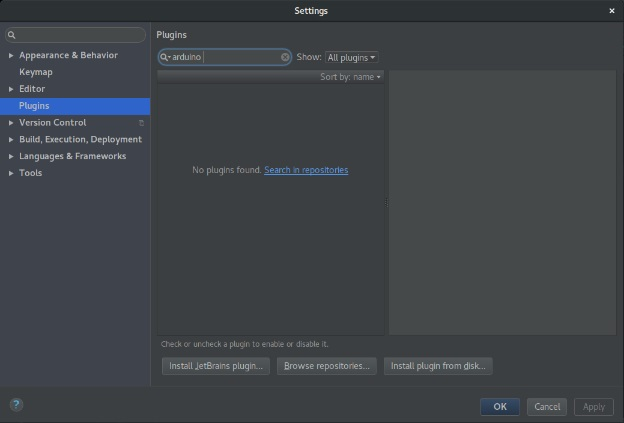
\includegraphics[width=0.5\textwidth]{pluginClion.jpg}
	\caption{Titulo.}
\end{figure}
\begin{figure}[H]	
	\centering
	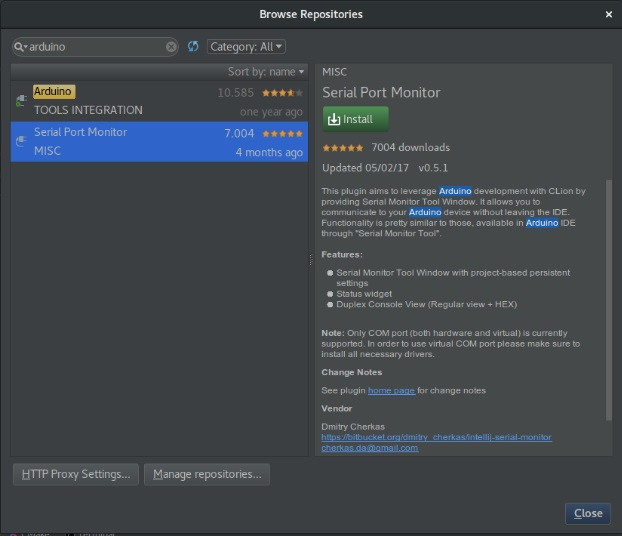
\includegraphics[width=0.5\textwidth]{pluginClion2.jpg}
	\caption{Titulo.}
\end{figure}
Após o final da instalação dos dois plugins reinicie o CLion para os plugins venham funcionar. Com a IDE aberta, no terminal, navegue com o comando ``CD" até o diretório do projeto o qual acabou de ser criado. Neste projeto foi criado a pasta TCCTerceira no diretório de projetos do CLion o qual se encontra na home do linux.
\begin{lstlisting}
cd /home/kelvimro/CLionProjects/TCCTerceira
\end{lstlisting}
Ainda no terminal é utilizado o comando ``platformio” com a opção ``boards”, este comando lista as placas de teste suportadas pelo PlatformIO.
\begin{lstlisting}
platformio boards
\end{lstlisting}
Ao localizar a placa desejada na lista, Arduino Nano processador Atmel 328, a qual foi escolhida para ser utilizada no desenvolvimento dos robôs de futebol do time UFMS-CPCX.
\begin{figure}[H]	
	\centering
	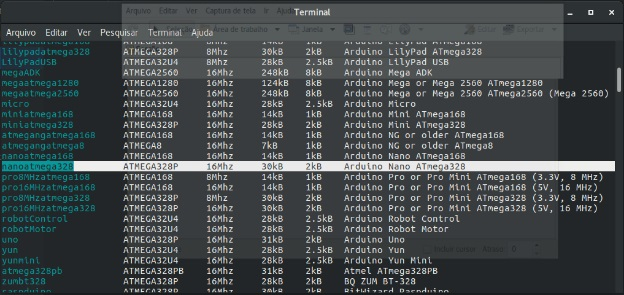
\includegraphics[width=0.5\textwidth]{boardPlatformio.jpg}
	\caption{Titulo.}
\end{figure}
Localizado e copiado o nome da placa ``nanoatmega328”, utilize o comando ``platformio” com as opções de ``init” para iniciar/instalar os recursos necessários no projeto,  a opção ``ide” deve-se ser utilizada o parâmetro ``clion" indicando que utilizamos o framework para trabalhar junto a IDE do Clion, sendo assim o comando completo utilizado foi:
\begin{lstlisting}
platformio init --ide clion --board nanoatmega328
\end{lstlisting}
\begin{figure}[H]	
	\centering
	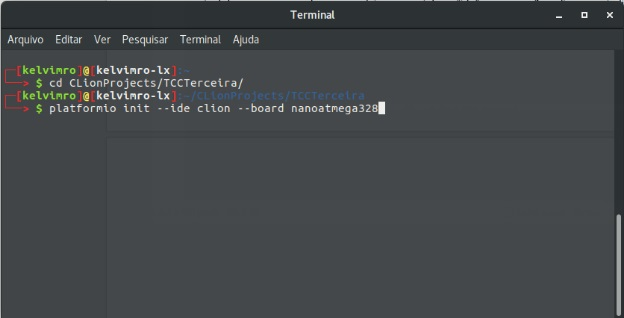
\includegraphics[width=0.5\textwidth]{initPlatformio.jpg}
	\caption{Titulo.}
\end{figure}
Finalizando a inicialização do PlatformIO será nescessário recarregar o arquivo CMake. Para isso clique com o botão direito do mouse em cima do nome do projeto(TCCTerceira) e em seguida em ``Reload CMake Project".
\begin{figure}[H]	
	\centering
	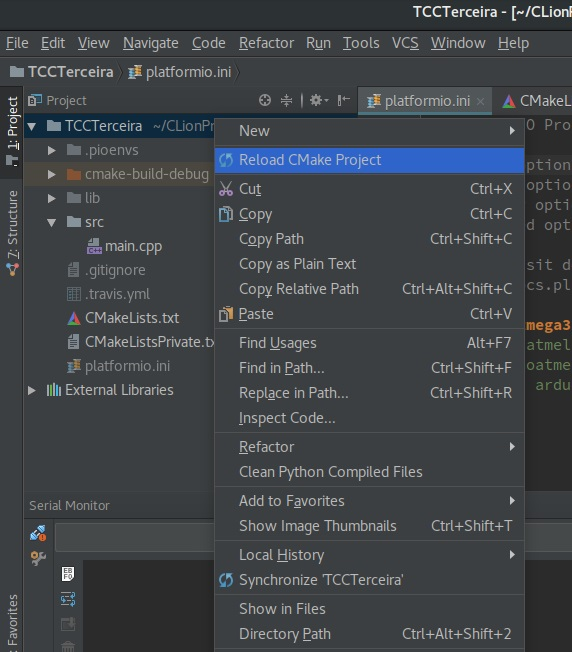
\includegraphics[width=0.5\textwidth]{reloadCmake.jpg}
	\caption{Titulo.}
\end{figure}
O PlatiformIO requer que as classes, assim como a Main.cpp, deve estar dentro da subpasta ``src" pois a ferramenta é configurada nativamente para buscar e compilar os códigos que ali estão. Na classe Main.cpp deve-se fazer o importe da biblioteca ``Arduino.h" por meio do ``\#include" a qual é a sintaxe para importar em C.
\begin{lstlisting}
#include <Arduino.h>
\end{lstlisting}
O código a seguir foi utilizado para teste de compilação e funcionamento do ambiente como um todo no fim da configuração. O programa tem a função básica, de piscar o led embutido na placa do arduino (LED\_BUILTIN) ou seja o pino da porta 13, ficando 1 segundo acesso e 1 segundo apagado.

\begin{lstlisting}
#include <Arduino.h>
void setup() {
// inicializa o pino digital LED_BUILTIN como saida.
pinMode(LED_BUILTIN, OUTPUT);
}

// Função loop do arduino
void loop() {
digitalWrite(LED_BUILTIN, HIGH);   // liga o LED 
delay(1000);                       // espera um segundo
digitalWrite(LED_BUILTIN, LOW);    // desliga o LED
delay(1000);                       // espera um segundo
}
\end{lstlisting}

Compilando o código utilizando Ctrl + F9 ou clicando no ícone no canto superior direito
\begin{figure}[H]	
	\centering
	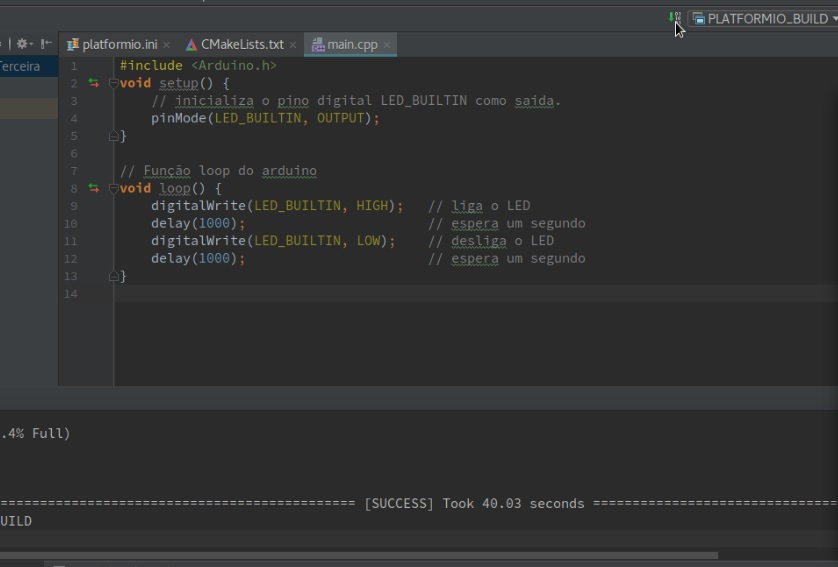
\includegraphics[width=0.5\textwidth]{buildClion.jpg}
	\caption{Titulo.}
\end{figure}
Ao receber a mensagem de ``SUCCESS" na aba ``Messages", indica que o ``build" ou seja, a compilação do programa foi concluída com exito.
No fim a compilação (build) é hora de subir(upload) do código para a placa arduino mudando para opção PLATFORMIO\_UPLOAD ( na caixa de seleção no canto superior direito) e clicando no ícone ``PLAY" verde.
\begin{figure}[H]	
	\centering
	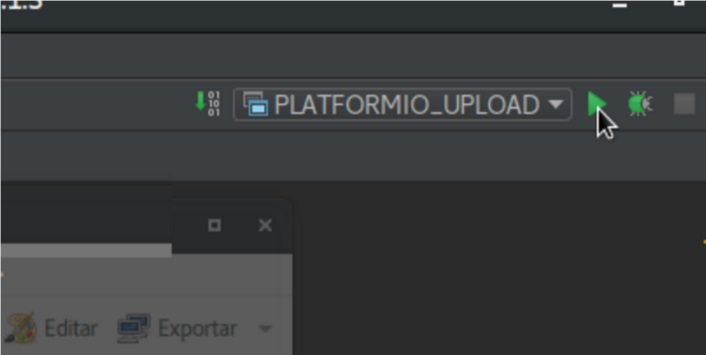
\includegraphics[width=0.5\textwidth]{upload.jpg}
	\caption{Titulo.}
\end{figure}
Aguarde a próxima mensagem de sucesso, a qual indicando que o programa já foi completamente enviado a placa, então o código já rodando.
ATENÇÃO: Algumas distribuições podem solicitar a permissão de administrador para ter acesso ao dispositivo USB antes de fazer o upload do código. O privilégio pode ser concedido com a utilização do comando:
\begin{lstlisting}
sudo chmod 777 /dev/ttyUSB0
\end{lstlisting}
Ps.: O numero “0” em ttyUSB0 deve ser trocado conforme a porta ao qual o dispositivo foi conectado.

Ps2.: Em algumas distribuições as permissões devem ser dadas sempre o dispositivo for conectado/reconectando.
Finalizando assim as configurações do ambiente de desenvolvimento, que foi utilizado para gerenciar e editar os códigos neste trabalho de conclusão.

\chapter{Controle Bluetooth}
Um simples projeto foi desenvolvido também em Arduino. O projeto tem a finalidade de ser um controle BT(Bluetooth) com um Joystick, utilizado para controlar as direções do robô. 
O joystick, um dos componentes do controle, nada mais é que dois potenciômetros, um potenciômetro para os valores do eixo X e outro para os valores do eixo Y. 
O controle possui um componente BT para estabelecer uma troca de dados junto ao robô, o qual também possui seu componente BT, o qual será explicado no capítulo <TeX>.
O código atualizado pode ser encontrado no link: https://github.com/kelvimro/TCCTerceira/blob/master/lib/ControleBT/controleBT.cpp 
O controle tem o intuito de simular os comandos que são gerados pela inteligência artificial no software que é responsável pelas táticas e movimento dos jogadores durante uma partida.
Os comandos podem variam entre -100 até 100, tendo um valor para cada motor, ou seja cada computação realizada pela inteligência artificial é enviado dois números inteiros, onde o primeiro número é destinado ao motor esquerdo e o segundo ao direito.
Utilizando-se da função map() a qual proporciona os valores do potenciômetro - dos quais variam entre 0 a 1023 - aos valores válidos para o robô.
\begin{lstlisting}
if (cmdX >= 0 && cmdX <= 501) cmdX = map(cmdX, 0, 501, -100, 0);
else cmdX = map(cmdX, 502, 1023, 0, 100);
if (cmdY >= 0 && cmdY <= 509) cmdY = map(cmdY, 0, 509, -100, 0);
else cmdY = map(cmdY, 510, 1023, 0, 100);
\end{lstlisting}
O potenciômetros Y, o qual vai representar os valores de potência, em posição neutra (sem ação do controlador) encontra-se com valor analógico de 509, então mapeado para 0, ou seja, não há potência requerida.
Ao movimentar o joystick para frente, aumenta-se o valor analogio do potenciômetro até o máximo de 1023 que após ter seu valor mapeado representa o valor 100.
Movimentando o joystick para trás, os valores analogicos lido diminuem até 0, denotando o valor -100. 
\begin{lstlisting}
if (cmdY >= 0 && cmdY <= 509) cmdY = map(cmdY, 0, 509, -100, 0);
else cmdY = map(cmdY, 510, 1023, 0, 100);
\end{lstlisting}
Valores positivos no eixo Y indicam que o movimento solicitado é para frente, enquanto os valores negativos representam movimento para trás.
O potenciômetros X, o qual vai representar os valores da diferença entre os motores. Em sua posição neutra tem o valor analogico lido de 502, representando 0\% de diferença entre os motores. Afim de facilitar a compreensão chamaremos de A o motor do lado esquerdo e de B o motor do lado direito. Então ao movimentar o joystick para a esquerda o valor analógico lido diminui até 0, resultando no valor de -100, movimentando o joystick para a direita aumentando o valor analógico lido até 1023 que representa o valor 100. 
\begin{lstlisting}
if (cmdX >= 0 && cmdX <= 501) cmdX = map(cmdX, 0, 501, -100, 0);
else cmdX = map(cmdX, 502, 1023, 0, 100);
\end{lstlisting}
No eixo X os valores negativos indicam que o motor A tem de se movimentar X\% mais lento em relação ao motor B, fazendo o movimento de curva para o lado de A. Já com os valores positivos de X indica que o motor B deve ser X\% mais lento q o A fazendo a curva para o lado B.


\chapter{Metodologia} \label{cap: metodologia}

\begin{enumerate}[(A)]
	
	\item Desenvolvimento e entrega do plano de trabalho;
	\item Escrita da introdução, levantamentos dos dados teóricos e bibliográficos.
	\item Revisão da literatura. 
	\item Implementar a aplicação
	\item Escritas do trabalho de conclusão do curso.		
	
	
\end{enumerate}


\begin{table}[!h]
	\renewcommand{\arraystretch}{1.3}
	\centering
	\begin{tabular}{|c|cccccccc|}
		%\hline
		%& \multicolumn{12}{c|}{Meses} \\
		\hline
		\multirow{2}{*}{\textbf{Etapas}} & \multicolumn{8}{c|}{\textbf{2017}} \\
		& \textbf{Abr} & \textbf{Jun} & \textbf{Jul} & \textbf{Ago} & \textbf{Set} & \textbf{Out} & \textbf{Nov} & \textbf{Dez}  \\
		\hline
		A & \checkmark & \checkmark & & & & & &  \\
		\hline
		B & & \checkmark & \checkmark & & & & &  \\
		\hline
		C & & & \checkmark & \checkmark & & & & \\
		\hline
		D & & & & \checkmark & \checkmark & \checkmark & &  \\
		\hline
		E & & & & & & & \checkmark & \checkmark \\
		\hline
	
		
	\end{tabular}
	\caption[Cronograma de atividades]{Cronograma de atividades.}
	\label{Tab:cronograma}
\end{table}

\chapter{Considerações Finais}


\vskip 10cm
\begin{table}[!h]
	\renewcommand{\arraystretch}{1.3}
	\centering
	\begin{tabular}{cccccccc}
		& & & & & & & \\
		Prof. Doc. Gedson Faria & & & & & & & Kelvim Rodrigues de Oliveira \\
		Orientador & & & & & & & Acadêmico \\
	\end{tabular}
\end{table}


\cleardoublepage
%\phantomsection
\addcontentsline{toc}{chapter}{Referências Bibliográficas} 
\bibliographystyle{abnt}
%\bibliographystyle{apalike} 
%\bibliographystyle{ieeetr} % Ordena por ordem de aparição.  
%\bibliographystyle{abbr} % Ordena por ordem alfabetica com nomes abreviados.
%\bibliographystyle{plain} % Ordena por ordem alfabetica com nomes por extenso.
\bibliography{bibliografia} % commented if *.bbl file included.

%\addcontentsline{toc}{chapter}{Ap\^endices}
%\appendix
%\include{apendice}

\end{document}